\documentclass[aspectratio=169,usenames,dvipsnames]{beamer}
\usepackage{graphicx}
\usepackage{multimedia}
\usepackage{media9}
\usepackage{url}
\usepackage[algoruled,vlined,linesnumbered]{algorithm2e}
%\usepackage{amsmath}
%\usepackage{amssymb}
\usepackage{latexsym}
\usepackage{multirow}
\usepackage{comment}
\usepackage{wasysym}
\usepackage{units}
\usepackage{wrapfig}
\usepackage{extarrows}
\usepackage{diagbox}
\usepackage{qtree}
\usepackage{booktabs}

%%%%%%%%%%%% My packages %%%%%%%%%%%%%%%%%%%%%%%%%%%%
\usepackage[symbol]{footmisc}
\usepackage{booktabs}

%\usepackage{longtable}
%\usepackage{float}
%\usepackage{colortbl}
%\usepackage{threeparttable}
%\usepackage{tabu}

\usepackage{MnSymbol}

% bibliography
\usepackage[backend=bibtex,style=authoryear]{biblatex}
\addbibresource{references.bib}

% define slide theme
%\usetheme{Boadilla}
\usetheme{default}

% MATLAB colors: https://www.mathworks.com/help/matlab/ref/matlab.graphics.chart.primitive.histogram-properties.html
\definecolor{m1}{rgb}{0,0.4470,0.7410}
\definecolor{m2}{rgb}{0.8500,0.3250,0.0980}
\definecolor{m3}{rgb}{0.9290,0.6940,0.1250}
\definecolor{m4}{rgb}{0.4940,0.1840,0.5560}
\definecolor{m5}{rgb}{0.4660,0.6740,0.1880}
\definecolor{m6}{rgb}{0.3010,0.7450,0.9330}
\definecolor{m7}{rgb}{0.6350,0.0780,0.1840}

\newcommand{\tcb}[1]{\textcolor{m1}{#1}}
\newcommand{\tco}[1]{\textcolor{m2}{#1}}
\newcommand{\tcv}[1]{\textcolor{m4}{#1}}
\newcommand{\tcg}[1]{\textcolor{m5}{#1}}
\newcommand{\tcm}[1]{\textcolor{m7}{#1}}

% define the heading color
\definecolor{myorange}{rgb}{0.807,0.3137,0.047}
\makeatletter
\colorlet{beamer@blendedblue}{myorange}
\makeatother

\definecolor{gray75}{gray}{0.75}

% define the footer
\definecolor{gray50}{gray}{0.5}
\setbeamertemplate{footline}[text line]{%
\parbox{\linewidth}{\vspace*{-8pt}\textcolor{gray50}{\inserttitle\hfill\insertpagenumber}}}

% get rid of the navigations symbols at the bottom
\setbeamertemplate{navigation symbols}{}

% custom font
%\usepackage{heuristica}
%\usepackage[heuristica,vvarbb,bigdelims]{newtxmath}
%\usepackage[T1]{fontenc}
%\renewcommand*\oldstylenums[1]{\textosf{#1}}
% More fonts here: http://www.tug.dk/FontCatalogue/mathfonts.html

%\usepackage[default]{comfortaa}
%\usepackage[T1]{fontenc}

\usepackage[sfdefault,light]{roboto}  
\usepackage[T1]{fontenc}


%%%%%%%%%%%%% Vadim's macro definitions %%%%%%%%%%%%%%%%%%

\newtheorem{df}{Definition}
\newtheorem{notation}{Notation}
\newtheorem{col}{Corollary}
\newtheorem{lem}{Lemma}

\newcommand{\td}{\,\nicefrac{\times}{\div}\,}

\newcommand{\bt}{\begin{theorem}\em}
\newcommand{\et}{\end{theorem}}
\newcommand{\Qed}{$\blacksquare$}
\renewcommand{\nin}{\noindent}
\newcommand{\bea}{\begin{eqnarray}}
\newcommand{\eea}{\end{eqnarray}}
\newcommand{\bdf}{\begin{df}\em}
\newcommand{\edf}{\end{df}}

\newcommand{\ben}{\begin{enumerate}}
\newcommand{\een}{\end{enumerate}}
\newcommand{\bei}{\begin{itemize}}
\newcommand{\eei}{\end{itemize}}
\newcommand{\ie}{\item}

\newcommand{\midb}{\pmb{\mid}}

\newcommand{\dist}{\operatorname{dist}}
\newcommand{\avg}{\operatornamewithlimits{avg}\limits}
\renewcommand{\arg}{\operatornamewithlimits{arg}\limits}
\newcommand{\round}{\operatorname{round}}
\newcommand{\lop}{\operatorname{lop}}
%\renewcommand{\min}{\operatornamewithlimits{argmin}\limits}
\renewcommand{\max}{\operatornamewithlimits{max}\limits}
\newcommand{\median}{\operatornamewithlimits{median}\limits}
\newcommand{\mean}{\operatornamewithlimits{mean}\limits}
\newcommand{\argmax}{\operatornamewithlimits{argmax}\limits}
\newcommand{\argmin}{\operatornamewithlimits{argmin}\limits}

\numberwithin{equation}{section}
\numberwithin{theorem}{section}
\numberwithin{lem}{section}
\numberwithin{df}{section}

\newcommand{\citea}[1]
{\citeauthor{#1} (\citeyear{#1})}

\setbeamerfont{caption}{series=\normalfont,size=\fontsize{6}{6}}
\definecolor{gray75}{gray}{0.75}
\setbeamertemplate{caption}{\raggedright\textcolor{myorange}{\insertcaption}\par}

\begin{document}

\title{Core Expansion in Optimization Crosswords}
\author{Adi Botea and Vadim Bulitko}
\institute{Eaton \& University of Alberta} 
%\institute{
\includegraphics[width=0.2\textwidth]{_template/uofa.pdf}} 

\date{July 15, 2023}

\frame{\titlepage} 

%%%%%%%%%%%%%%%%%%%%%%%%%%%%%%%%%%%%%%%%%%%%%%%%%%%%%%%%%%%%%%%%%%%%%%%%%%%%%%%%

\begin{frame}{Outline}

\bei

\ie Problem

\bigskip

\ie Contribution

\bigskip

\ie Related Work

\bigskip

\ie Approach

\bigskip

\ie Results

\bigskip

\ie Conclusions

\eei

\end{frame}

%%%%%%%%%%%%%%%%%%%%%%%%%%%%%%%%%%%%%%%%%%%%%%%%%%%%%%%%%%%%%%%%%%%%%%%%%%%%%%%%

\begin{frame}{Romanian Crosswords Competition ({\sc Roco})}

\begin{columns}
\column{0.6\linewidth}
\bei
\ie Annual competition: 1965 to present
\bei 
\ie top 12 human-submitted grids published
\eei

\bigskip

\ie Input: word lists
\bei
\ie regular Romanian words (about $134$K)
\ie thematic words, vary per year (e.g., $387$)
\eei

\bigskip

\ie Task:
\bei 
\ie build a $13\times13$ grid filled with words
\bei
\ie some constraints
\eei
\ie score = sum of lengths of all thematic words
\eei

\eei

\column{0.4\linewidth}
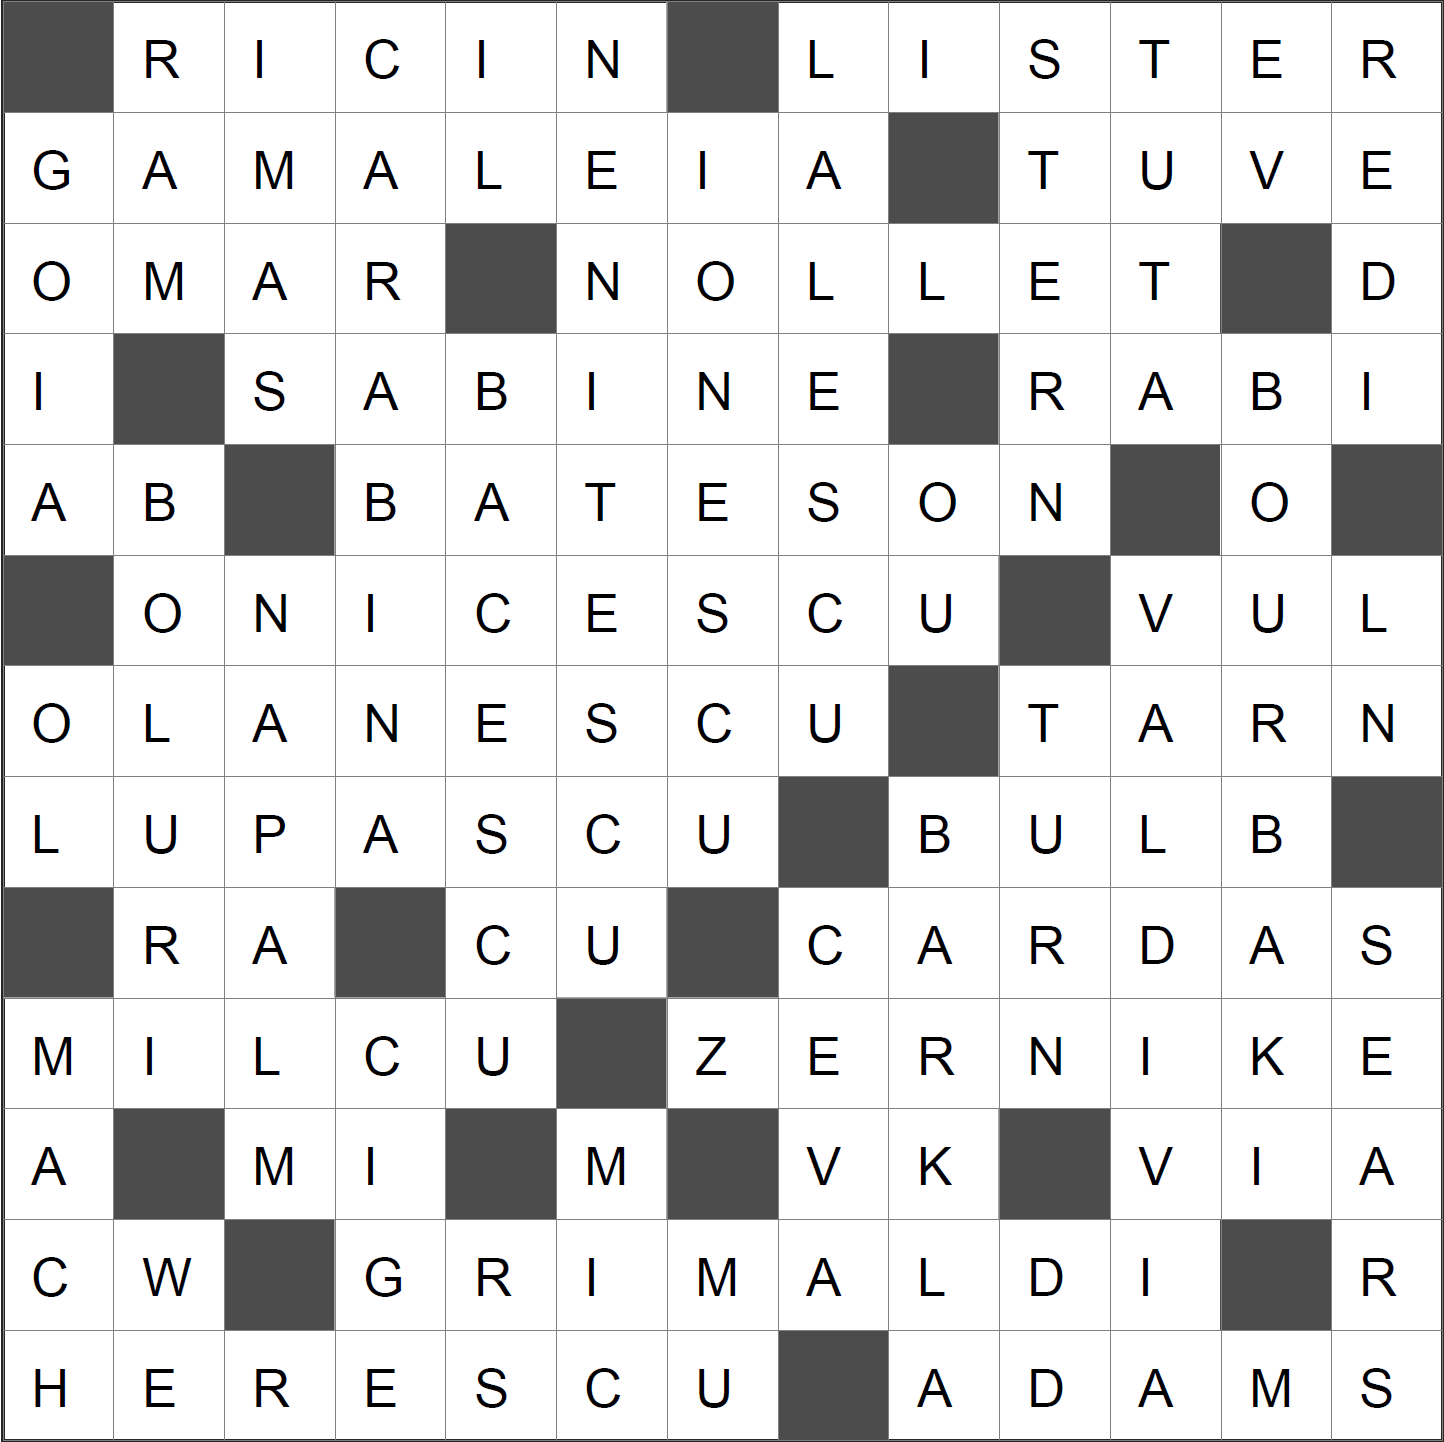
\includegraphics[width=\columnwidth]{figs/2013b.png}
\end{columns}
\end{frame}

%%%%%%%%%%%%%%%%%%%%%%%%%%%%%%%%%%%%%%%%%%%%%%%%%%%%%%%%%%%%%%%%%%%%%%%%%%%%%%%%

\begin{frame}{Primary Contribution}

\bei

\ie \tcm{AI used to lag behind the top-12 scores~[\cite{DBLP:conf/cig/BulitkoB21}]}

\bigskip

\bigskip


\ie \tcg{Our approach entered top-12 range in each of the three years tried}

\eei

\end{frame}


%%%%%%%%%%%%%%%%%%%%%%%%%%%%%%%%%%%%%%%%%%%%%%%%%%%%%%%%%%%%%%%%%%%%%%%%%%%%%%%%

\begin{frame}{Related Work}

\bei

\ie \tcm{Adi: please write, use {\tt [$\backslash$cite]} for citations}

\eei

\end{frame}

%%%%%%%%%%%%%%%%%%%%%%%%%%%%%%%%%%%%%%%%%%%%%%%%%%%%%%%%%%%%%%%%%%%%%%%%%%%%%%%%

\begin{frame}{Our Approach: Intuition}

\bei

\ie \tcb{naive approach} 
\bei 
\ie try different combinations of $26$ black cells on a $13 \times 13$ grid
\ie fill in each with words via {\sc Wombat}
\ie compute the score
\ie select the best
\eei

\bigskip

\ie \tcm{problems}
\bei
\ie filling a configuration of $26$ black cells with words takes minutes
\ie thus, only a small number of such combinations can be filled in
\ie needle in a hay stack...
\eei

\bigskip

\ie \tcg{proposed solution}
\bei
\ie start with a cluster of thematic words $\to$ guaranteed score points
\ie build the rest of the grid around it
\eei

\eei

\end{frame}




%%%%%%%%%%%%%%%%%%%%%%%%%%%%%%%%%%%%%%%%%%%%%%%%%%%%%%%%%%%%%%%%%%%%%%%%%%%%%%%%


\begin{frame}{Our Approach: Overview}

\begin{columns}
\column{0.7\linewidth}

\bei
\ie build cores from a pattern (human input)

\medskip

\ie build expanded cores

\medskip

\ie build seeds

\medskip

\ie develop seeds into full solutions
\bei
\ie select promising seeds 
\ie complete them to full grids filled with words
\eei
\eei

\column{.3\linewidth}

\begin{figure}
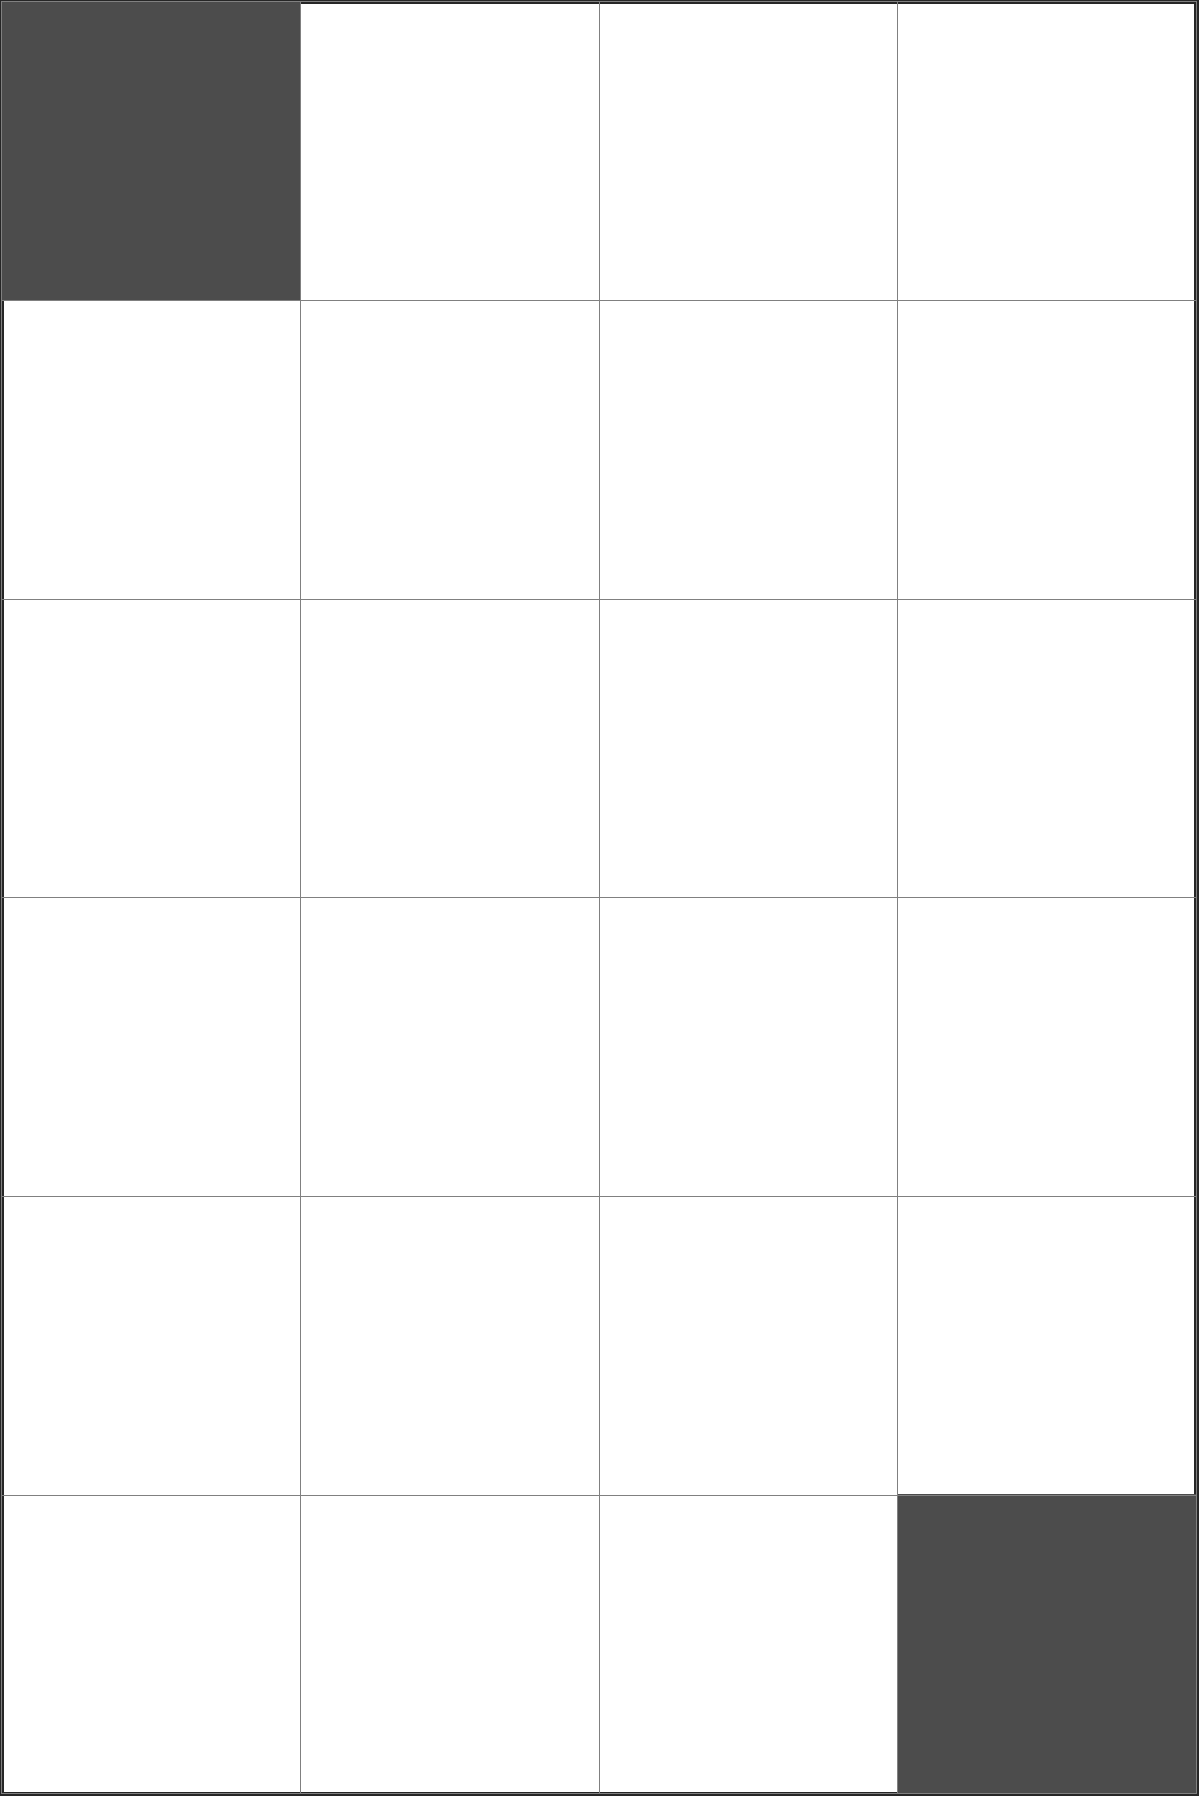
\includegraphics[width=0.7\columnwidth]{_plots/6x4-puzzle.png}
\vspace{-0.25cm}
\caption{{\bf pattern}: a rectangular grid with no letters}
\end{figure}

\end{columns}

\end{frame}

%%%%%%%%%%%%%%%%%%%%%%%%%%%%%%%%%%%%%%%%%%%%%%%%%%%%%%%%%%%%%%%%%%%%%%%%%%%%%%%%


\begin{frame}{Patterns $\to$ Cores}

\begin{columns}
\column{0.7\linewidth}

\bei
\ie construct a small puzzle
\bei 
\ie the grid is the pattern
\eei

\bigskip

\ie feed the puzzle into {\sc Wombat}~[\cite{DBLP:conf/socs/BoteaB21}]
\bei 
\ie the dictionary contains substrings of thematic words
\ie generate multiple solutions 
\ie each solution is the core
\eei
\eei

\column{.3\linewidth}

\begin{figure}
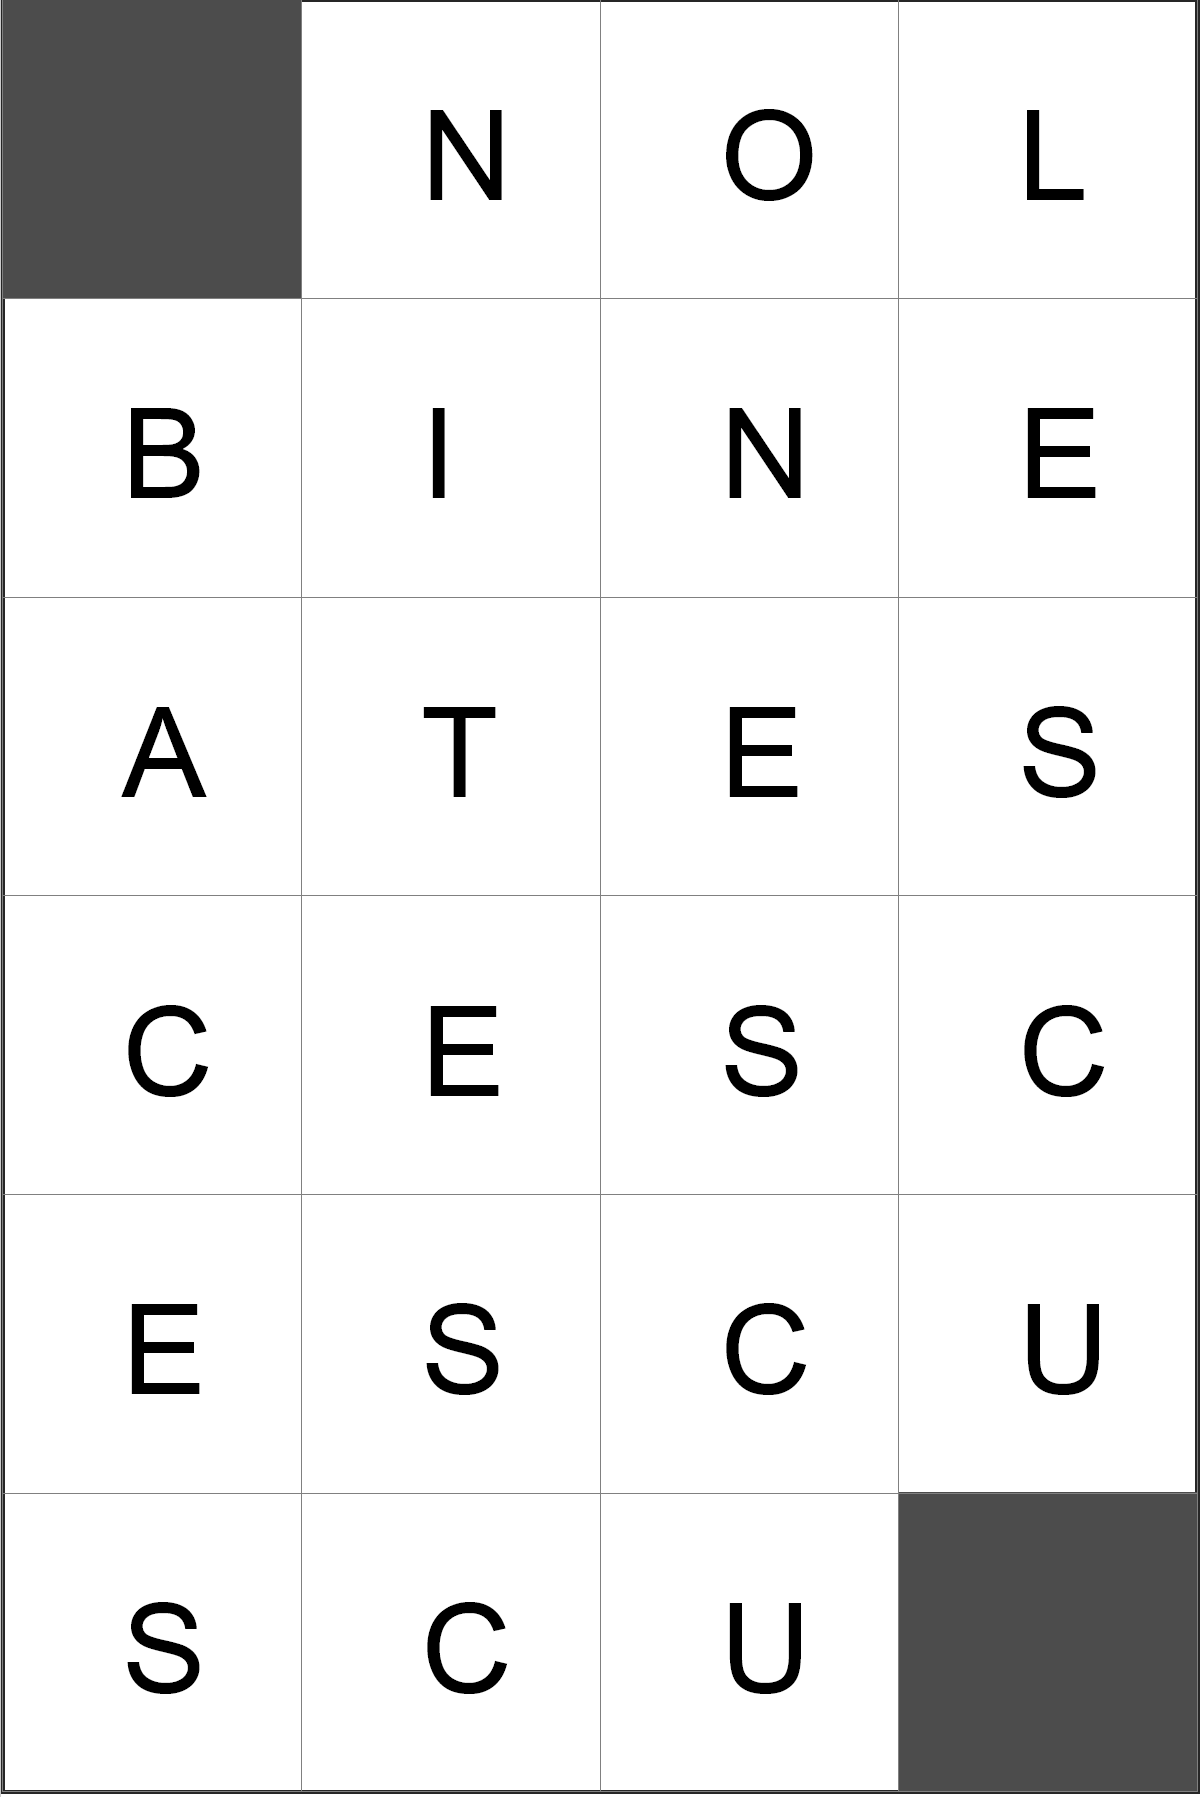
\includegraphics[width=0.7\columnwidth]{_plots/core-6x4-puzzle.png}
%\vspace{-0.15cm}
\caption{{\bf core}: a pattern filled with letters. Each word is a substring of a thematic word}
\end{figure}

\end{columns}

\end{frame}

%%%%%%%%%%%%%%%%%%%%%%%%%%%%%%%%%%%%%%%%%%%%%%%%%%%%%%%%%%%%%%%%%%%%%%%%%%%%%%%%


\begin{frame}{Cores $\to$ Expanded Cores}

\begin{columns}
\column{0.5\linewidth}

\bei
\ie match full thematic words to strings in the core

\medskip

\ie depth first search \tcm{Adi: need more here}
\eei

\column{.5\linewidth}

\begin{figure}
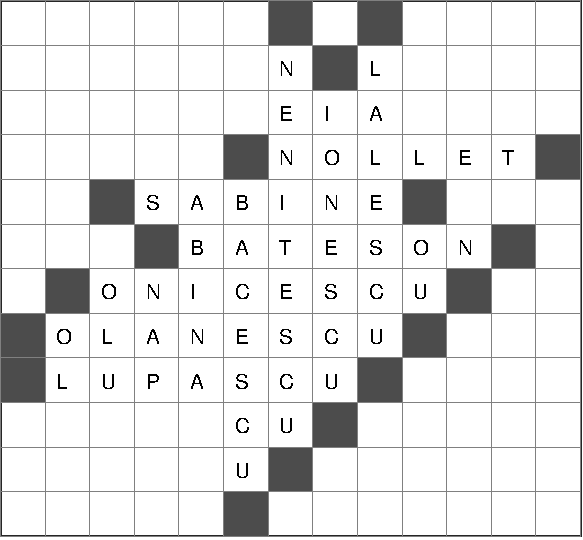
\includegraphics[width=0.9\columnwidth]{_plots/extcore-alive-0-puzzle-72-2975-1488--1--1.pdf}
%\vspace{-0.15cm}
\caption{{\bf expanded core}: a rectangular grid with white cells, black cells and white cells with letters. Contains full thematic words bookended with black cells}
\end{figure}

\end{columns}

\end{frame}

%%%%%%%%%%%%%%%%%%%%%%%%%%%%%%%%%%%%%%%%%%%%%%%%%%%%%%%%%%%%%%%%%%%%%%%%%%%%%%%%

\begin{frame}{Expanded Cores $\to$ Seeds}

\begin{columns}
\column{0.5\linewidth}

\bei
\ie place an expanded core inside a $13\times13$ grid

\medskip

\ie shift horizontally and vertically to obtain multiple seeds

\medskip

\ie prune away seeds proven illegal \tcm{Adi: dead seeds? Illegal seeds?}
\eei

\column{.5\linewidth}

\begin{figure}
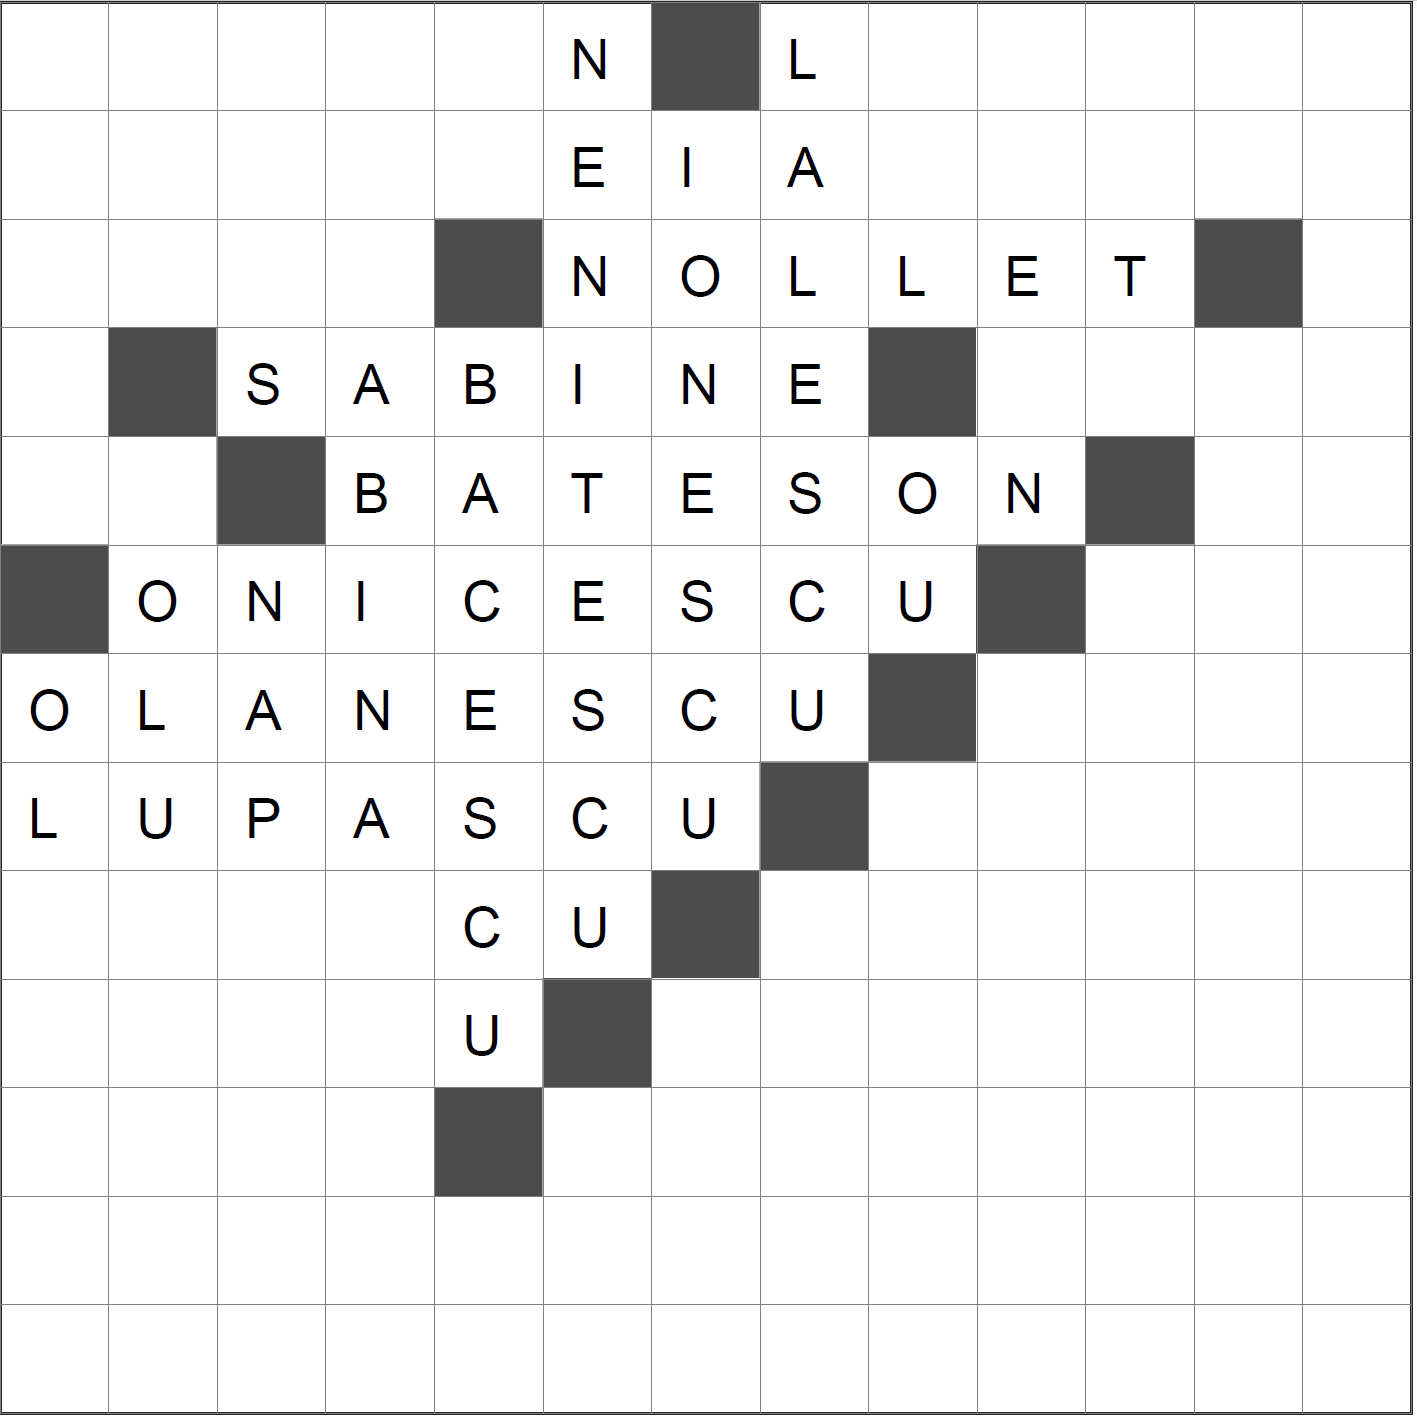
\includegraphics[width=0.9\columnwidth]{_plots/alive-0-puzzle-72-2975-1488--1--1.png}
\vspace{-0.25cm}
\caption{{\bf seed}: a $13\times13$ grid with white cells, black cells and white cells with letters}
\end{figure}

\end{columns}

\end{frame}

%%%%%%%%%%%%%%%%%%%%%%%%%%%%%%%%%%%%%%%%%%%%%%%%%%%%%%%%%%%%%%%%%%%%%%%%%%%%%%%%


\begin{frame}{Full Sequence: Pattern $\rightarrow$ Core $\rightarrow$ Expanded core $\rightarrow$ Seed}

\begin{figure}
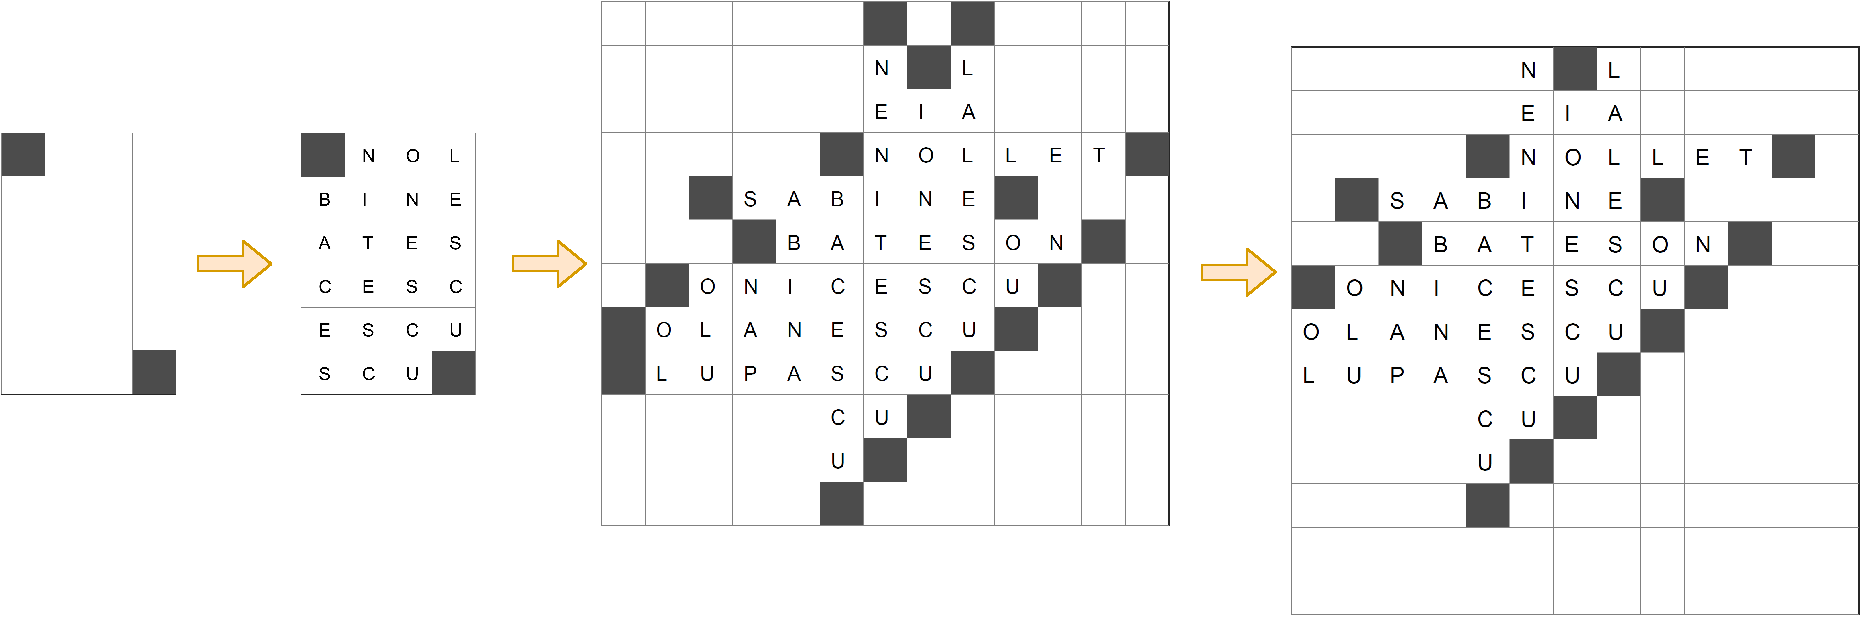
\includegraphics[width=\textwidth]{figs/4part.pdf}
\caption{the stages are aligned vertically to illustrate how the expansion and build happen. Note, for instance, how the partial word ``NOL'' becomes ``NOLLET''. }
\label{fig:pattern}
\end{figure}

\end{frame}

%%%%%%%%%%%%%%%%%%%%%%%%%%%%%%%%%%%%%%%%%%%%%%%%%%%%%%%%%%%%%%%%%%%%%%%%%%%%%%%%

\begin{frame}{What is Next?}

\bei

\ie seeds themselves have very low scores due to empty spaces

\bigskip
\bigskip

\ie need to complete them
\bei
\ie place the remaining black cells (up to $26$)
\ie fill words in the resulting slots
\ie do not disturb the score-yielding part
\eei


\eei


\end{frame}

%%%%%%%%%%%%%%%%%%%%%%%%%%%%%%%%%%%%%%%%%%%%%%%%%%%%%%%%%%%%%%%%%%%%%%%%%%%%%%%%

\begin{frame}{Selecting Promising Seeds to Complete}

\bei

\ie trying to complete each seed is too expensive

\bigskip
\bigskip

\ie select promising seeds via Monte Carlo
\bei
\ie for each seed place additional black cells in the empty area
\ie quickly run {\sc Wombat} on it 
\ie repeat until per-seed time budget is exhausted
\ie the maximum score of each rollout is the seed's MC score
\eei

\bigskip
\bigskip

\ie could use such MC seed completions as the final solution
\bei
\ie MC rollouts do not allow incremental improvements
\ie insufficiently high scores
\eei

\eei


\end{frame}

%%%%%%%%%%%%%%%%%%%%%%%%%%%%%%%%%%%%%%%%%%%%%%%%%%%%%%%%%%%%%%%%%%%%%%%%%%%%%%%%

\begin{frame}{Evolving Promising Seeds Into Full Solutions}

\bei

\ie sort all seeds by their MC scores

\bigskip
\bigskip

\ie complete the top $N$ seeds via incremental improvements
\bei
\ie can use various search techniques
\ie the space is large so stochastic searches are promising
\ie standard genetic algorithms risk a population collapse
\ie we use a version of MAP-Elites~[\cite{mapElites}]
\bei
\ie maintains diversity explicitly
\ie via the use of maps
\eei
\eei

\eei


\end{frame}

%%%%%%%%%%%%%%%%%%%%%%%%%%%%%%%%%%%%%%%%%%%%%%%%%%%%%%%%%%%%%%%%%%%%%%%%%%%%%%%%

\begin{frame}{MAP-Elites}

\bei

\ie MAP-Elites stores its population in a map
\bei
\ie a map is a 2D table
\ie each row and column correspond to feature values
\bei
\ie maximum word slot length ($f_1$)
\ie number of walls ($f_2$)
\eei
\ie elites from different cells do not compete
\eei
\ie on each generation a few elites are randomly picked from each map
\ie each elite is mutated (seed area protected)
\ie each offspring is run through {\sc Wombat} (higher time limit)
\ie a scored offspring replaces an existing elite if its score is higher
\eei

\end{frame}


%%%%%%%%%%%%%%%%%%%%%%%%%%%%%%%%%%%%%%%%%%%%%%%%%%%%%%%%%%%%%%%%%%%%%%%%%%%%%%%%

\begin{frame}{Multi-map MAP-Elites}

\bei

\ie how large should the maps/tables be?
\bei
\ie too many cells $\to$ little competition
\bei
\ie every one is a champion in its own niche
\eei

\ie too few cells $\to$ too much competition
\bei
\ie danger of collapsing to a single individual
\eei
\eei

\bigskip

\ie we used three maps
\bei
\ie by using different resolution of feature ranges
\eei

\eei

\begin{table}
{\small\centering
\begin{tabular}{c|c|c|c}
\toprule
{\bf map} & {\bf $f_1$ values} & {\bf $f_2$ values} & {\bf map size} \\
\midrule
$1$ & $\{6,9.5,13\}$ & $\{0,13,26\}$ & $3 \times 3$ \\
$2$ & $\{6,8.3333,10.667,13\}$ & $\{0,2,4,\dots,26\}$ & $4 \times 14$\\
$3$ & $\{6,7,\dots,13\}$ & $\{0,1,\dots,26\}$ & $8 \times 27$\\
\bottomrule
\end{tabular}}
\caption{Feature values in our multi-map MAP-Elites algorithm}
\label{tab:mrme}
\end{table}

\end{frame}


%%%%%%%%%%%%%%%%%%%%%%%%%%%%%%%%%%%%%%%%%%%%%%%%%%%%%%%%%%%%%%%%%%%%%%%%%%%%%%%%

\begin{frame}{Experiments}

\begin{table}[htbp]
{\footnotesize\centering
\begin{tabular}{c|r|r|r|r|r|r|r}
\toprule
{\bf year} & {\bf cores} & {\bf expanded} & {\bf seeds} & {\bf seeds} & {\bf ranking} & {\bf seeds} & {\bf evolving}\\
           & & {\bf cores} & {\bf before} & {\bf ranked} & {\bf time} & {\bf evolved} & {\bf time} \\
           & & & {\bf postprocessing} & {\bf ($N$)} & & {\bf ($K$)} & \\
\midrule
2013 & $12,\!560$ & $2,\!754$ & $1,\!259$ & $932$ & $30$ minutes & $352$ & $1.9$ days \\ 
2021 & $332,\!062$ & $1,\!005,\!114$ & $122,\!579$ & $38,\!035$ & $21$ hours & $224$ & $1.2$ days \\ 
2023 & $123,\!218$ & $1,\!042$ & $1,\!087$ & $446$ & $16$ minutes & $352$ & $2.0$ days \\ 
\bottomrule
\end{tabular}}
\end{table}


\end{frame}

%%%%%%%%%%%%%%%%%%%%%%%%%%%%%%%%%%%%%%%%%%%%%%%%%%%%%%%%%%%%%%%%%%%%%%%%%%%%%%%%

\begin{frame}{Results}

\begin{figure}
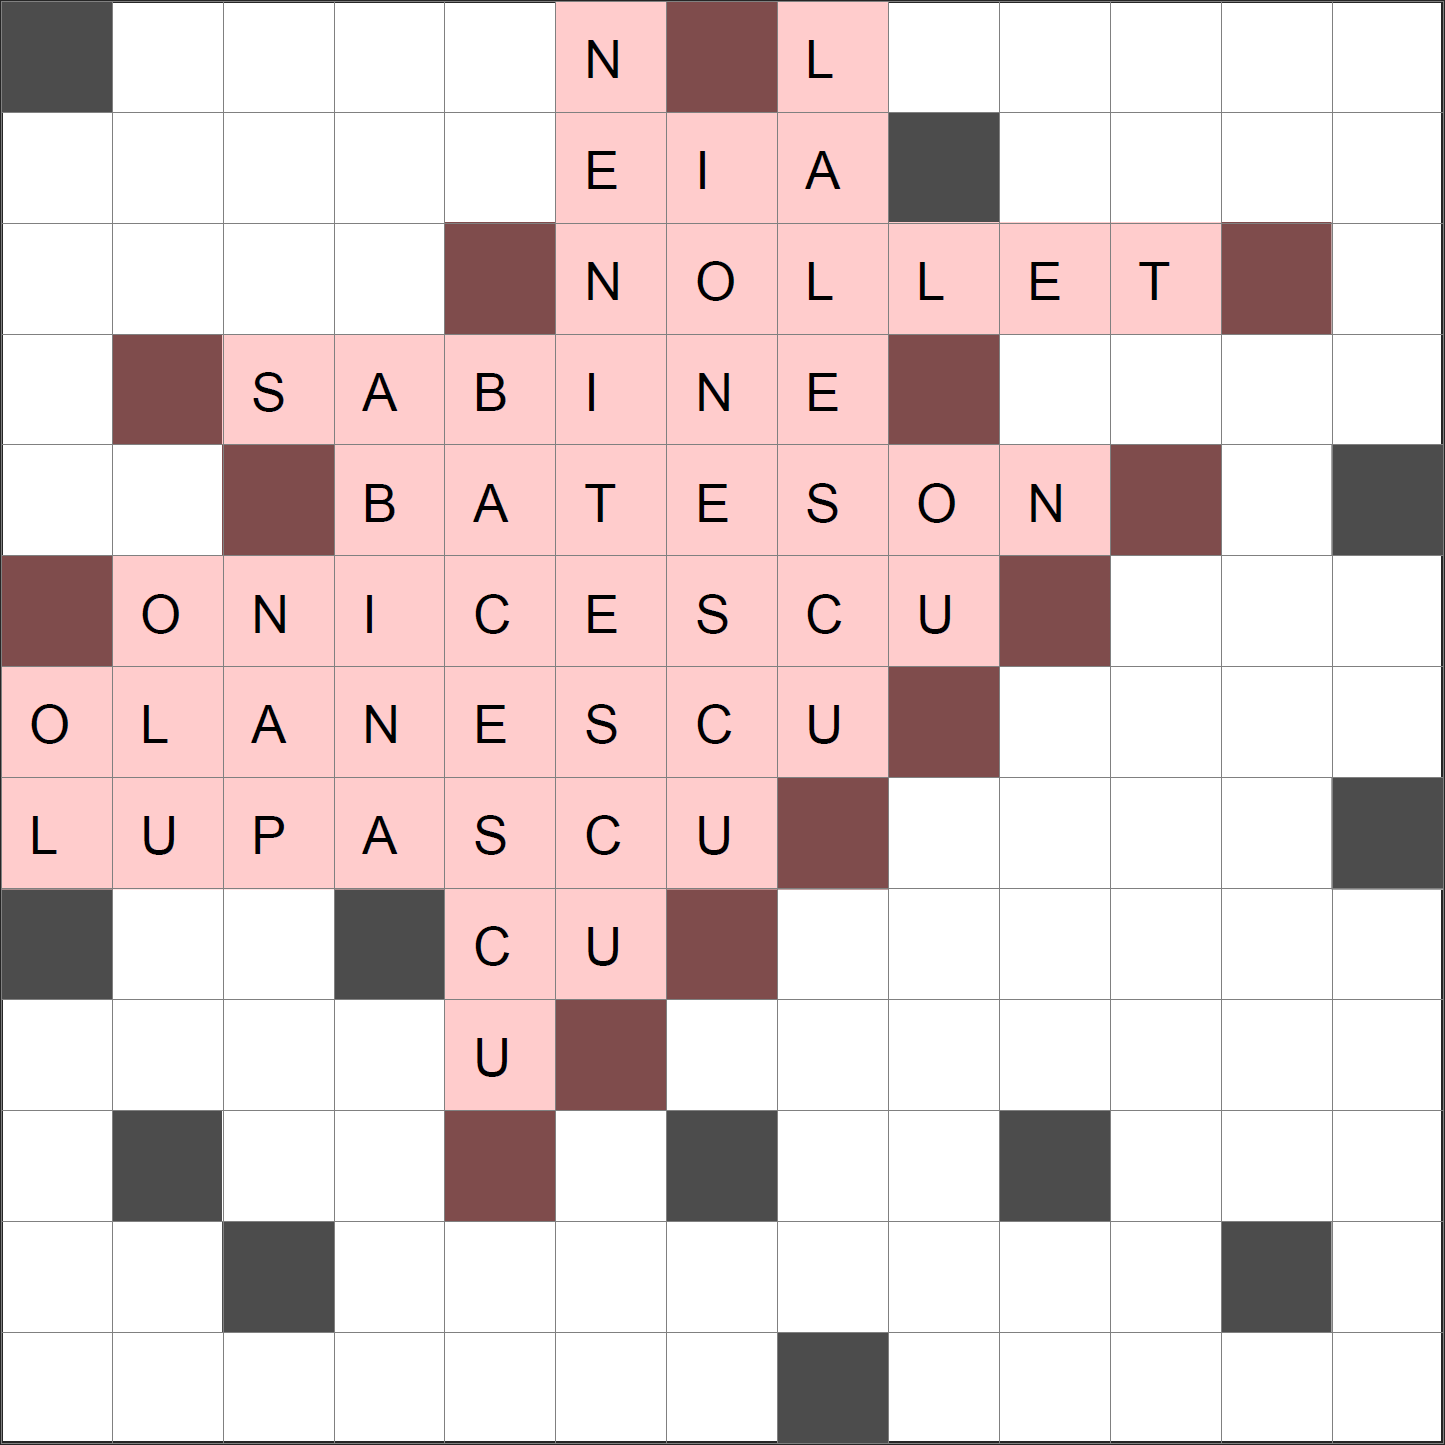
\includegraphics[height=3.1cm]{figs/2013a.png}
%
\hspace{1cm}
%
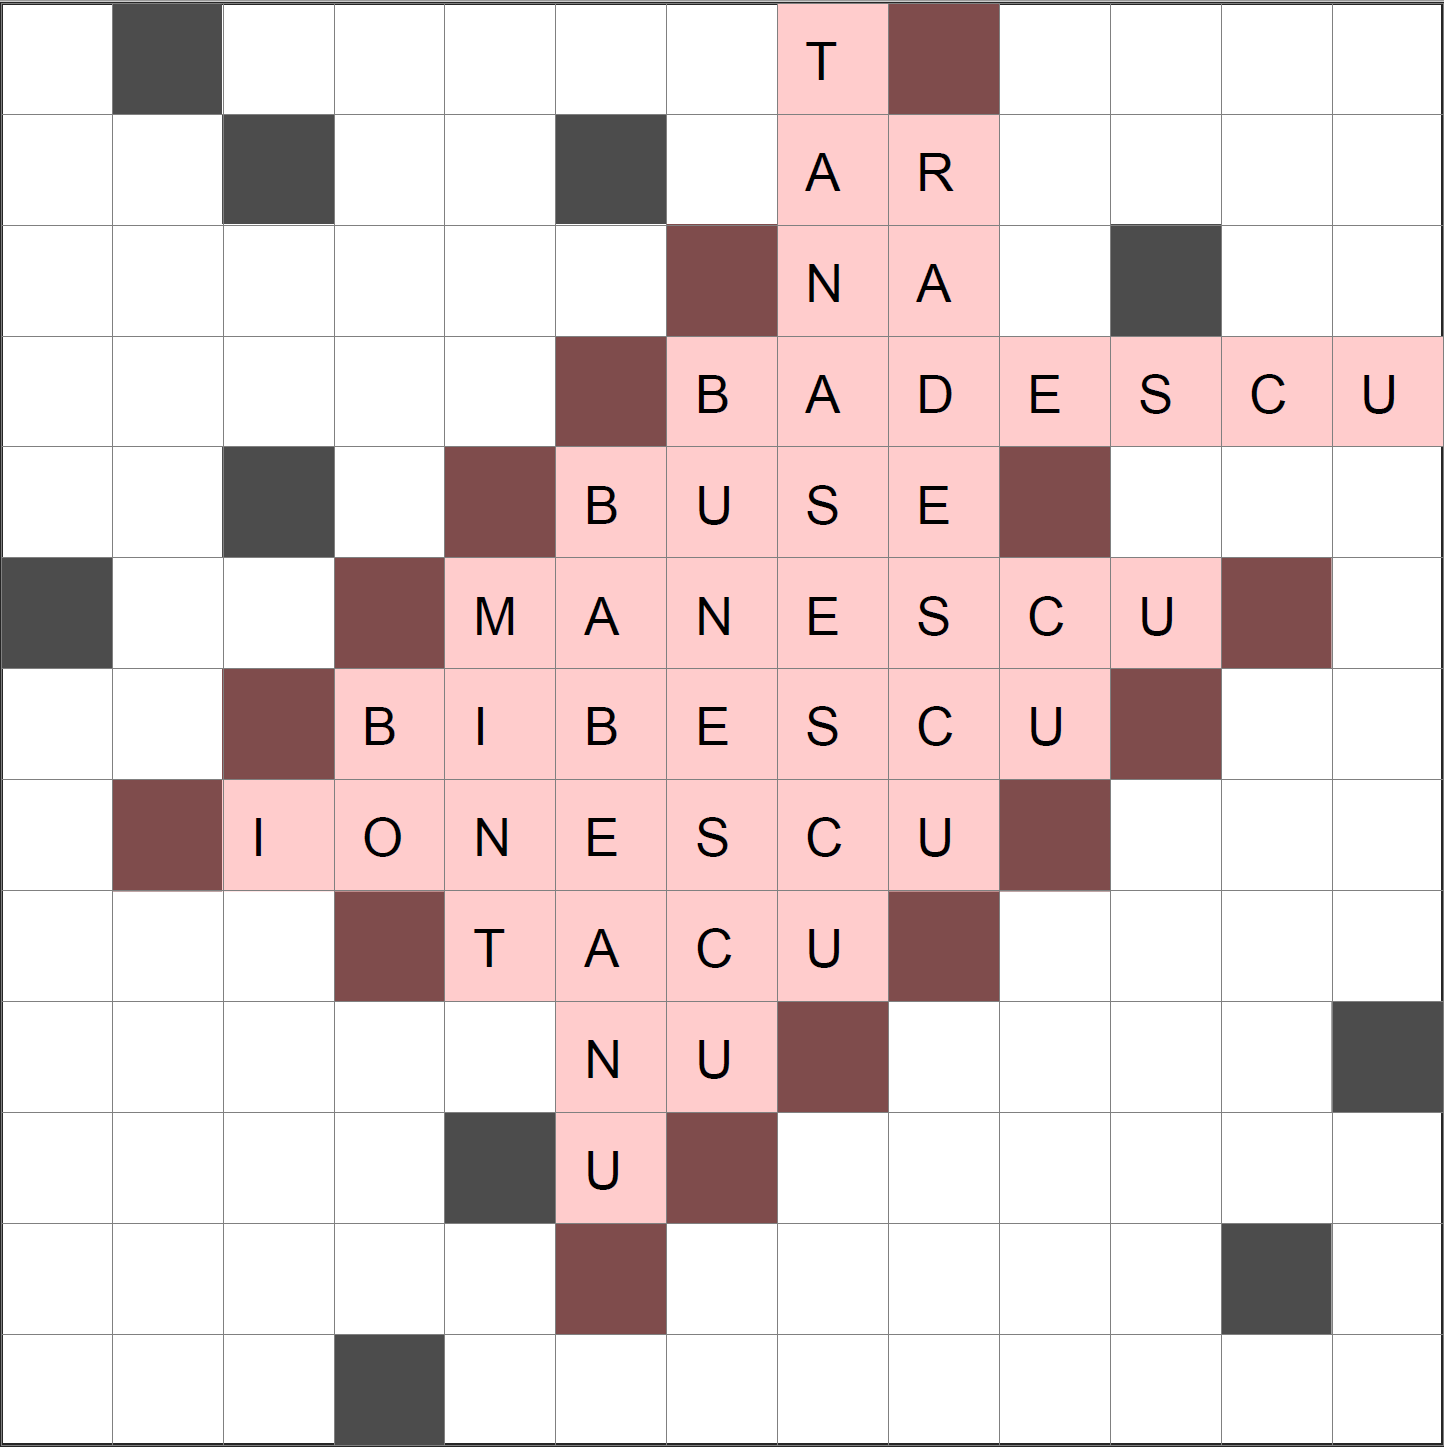
\includegraphics[height=3.1cm]{figs/2021a.png}
%
\hspace{1cm}
%
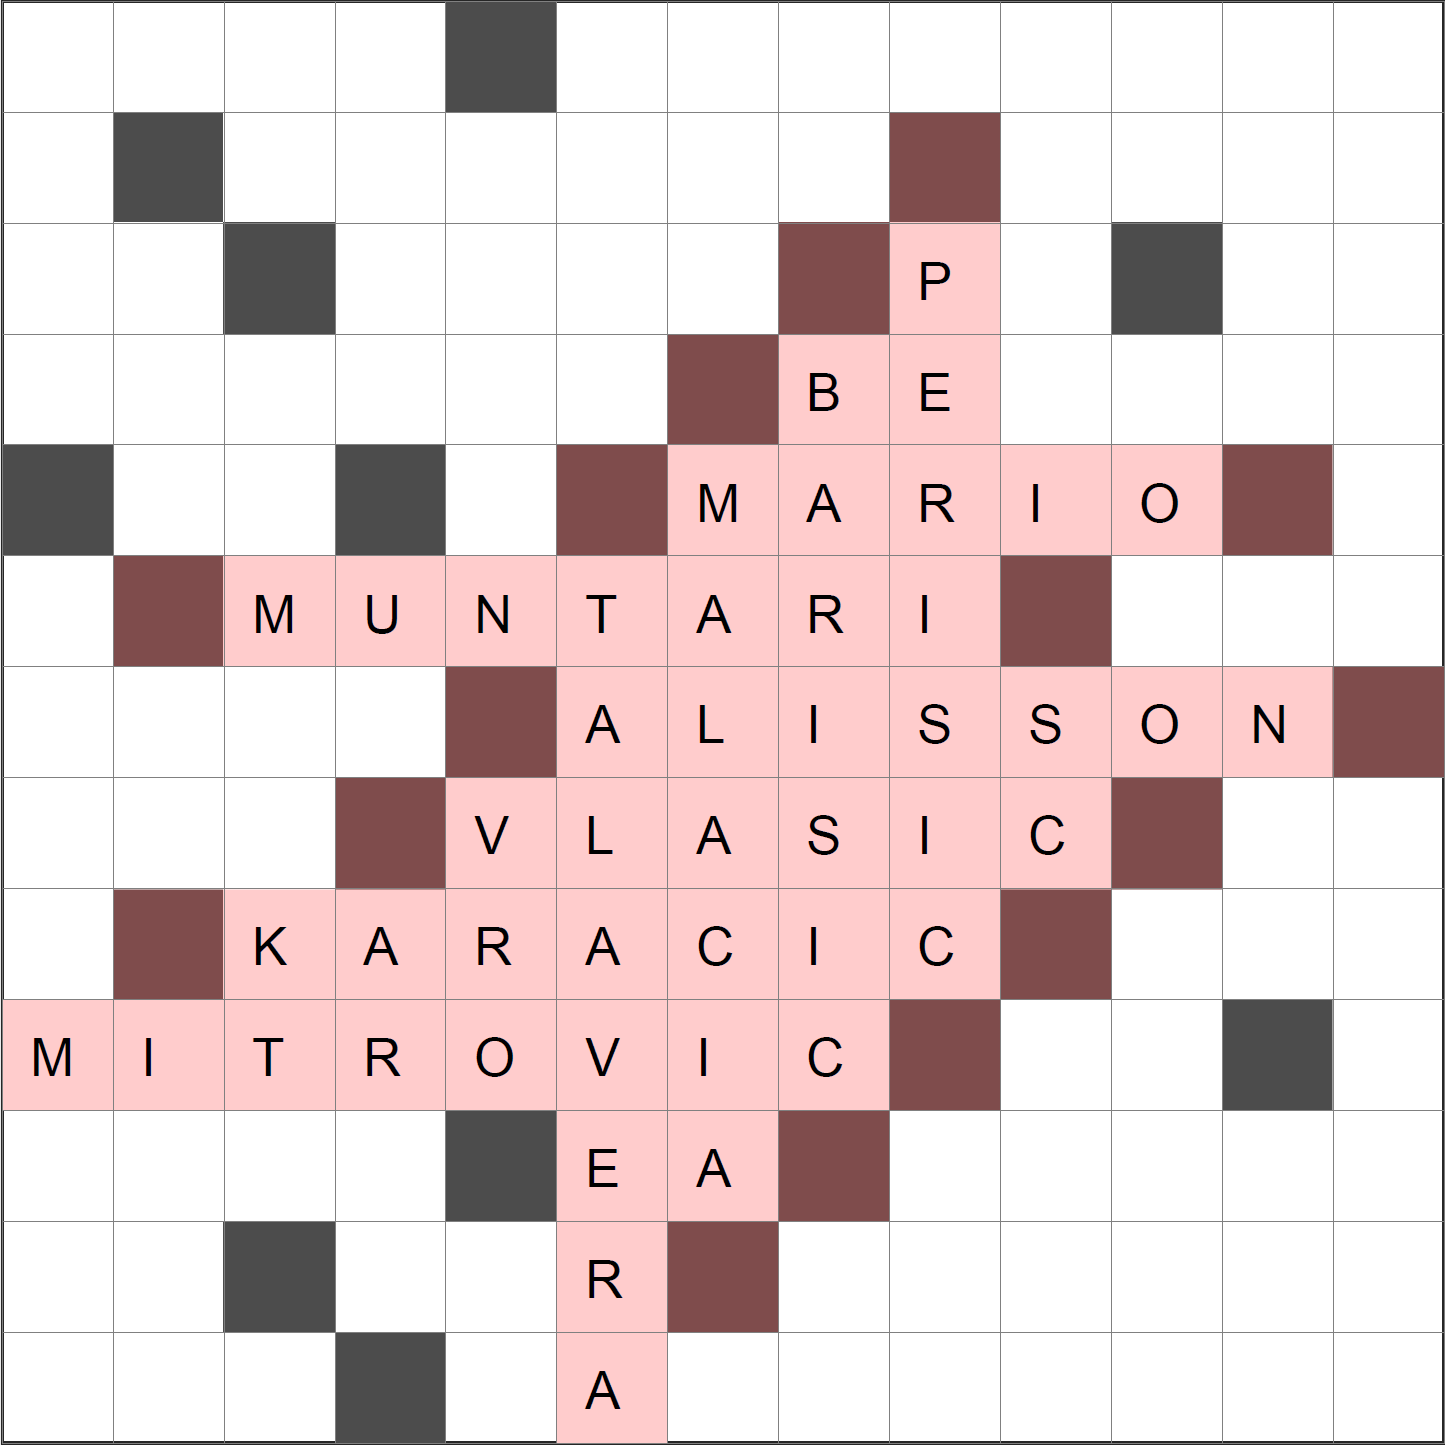
\includegraphics[height=3.1cm]{figs/2023a.png}

\vspace{0.25cm}

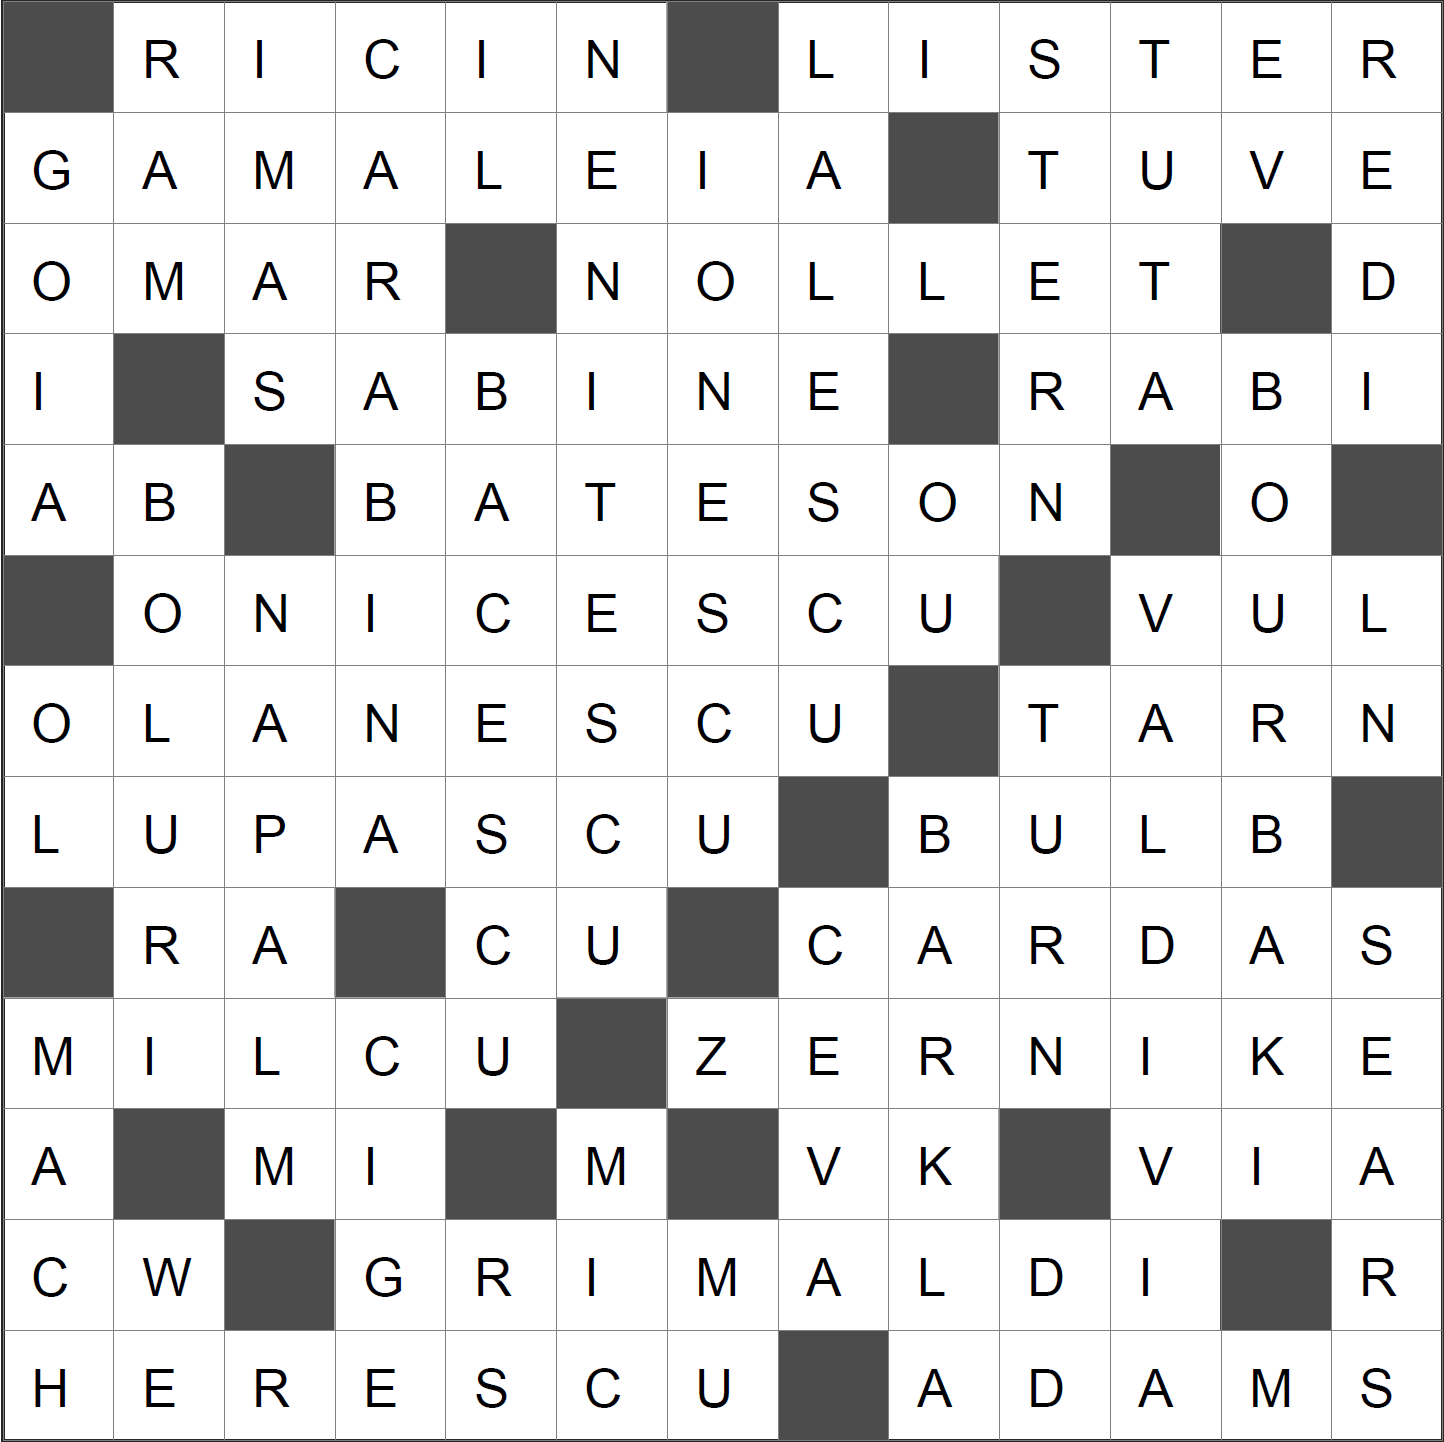
\includegraphics[height=3.1cm]{figs/2013b.png}
%
\hspace{1cm}
%
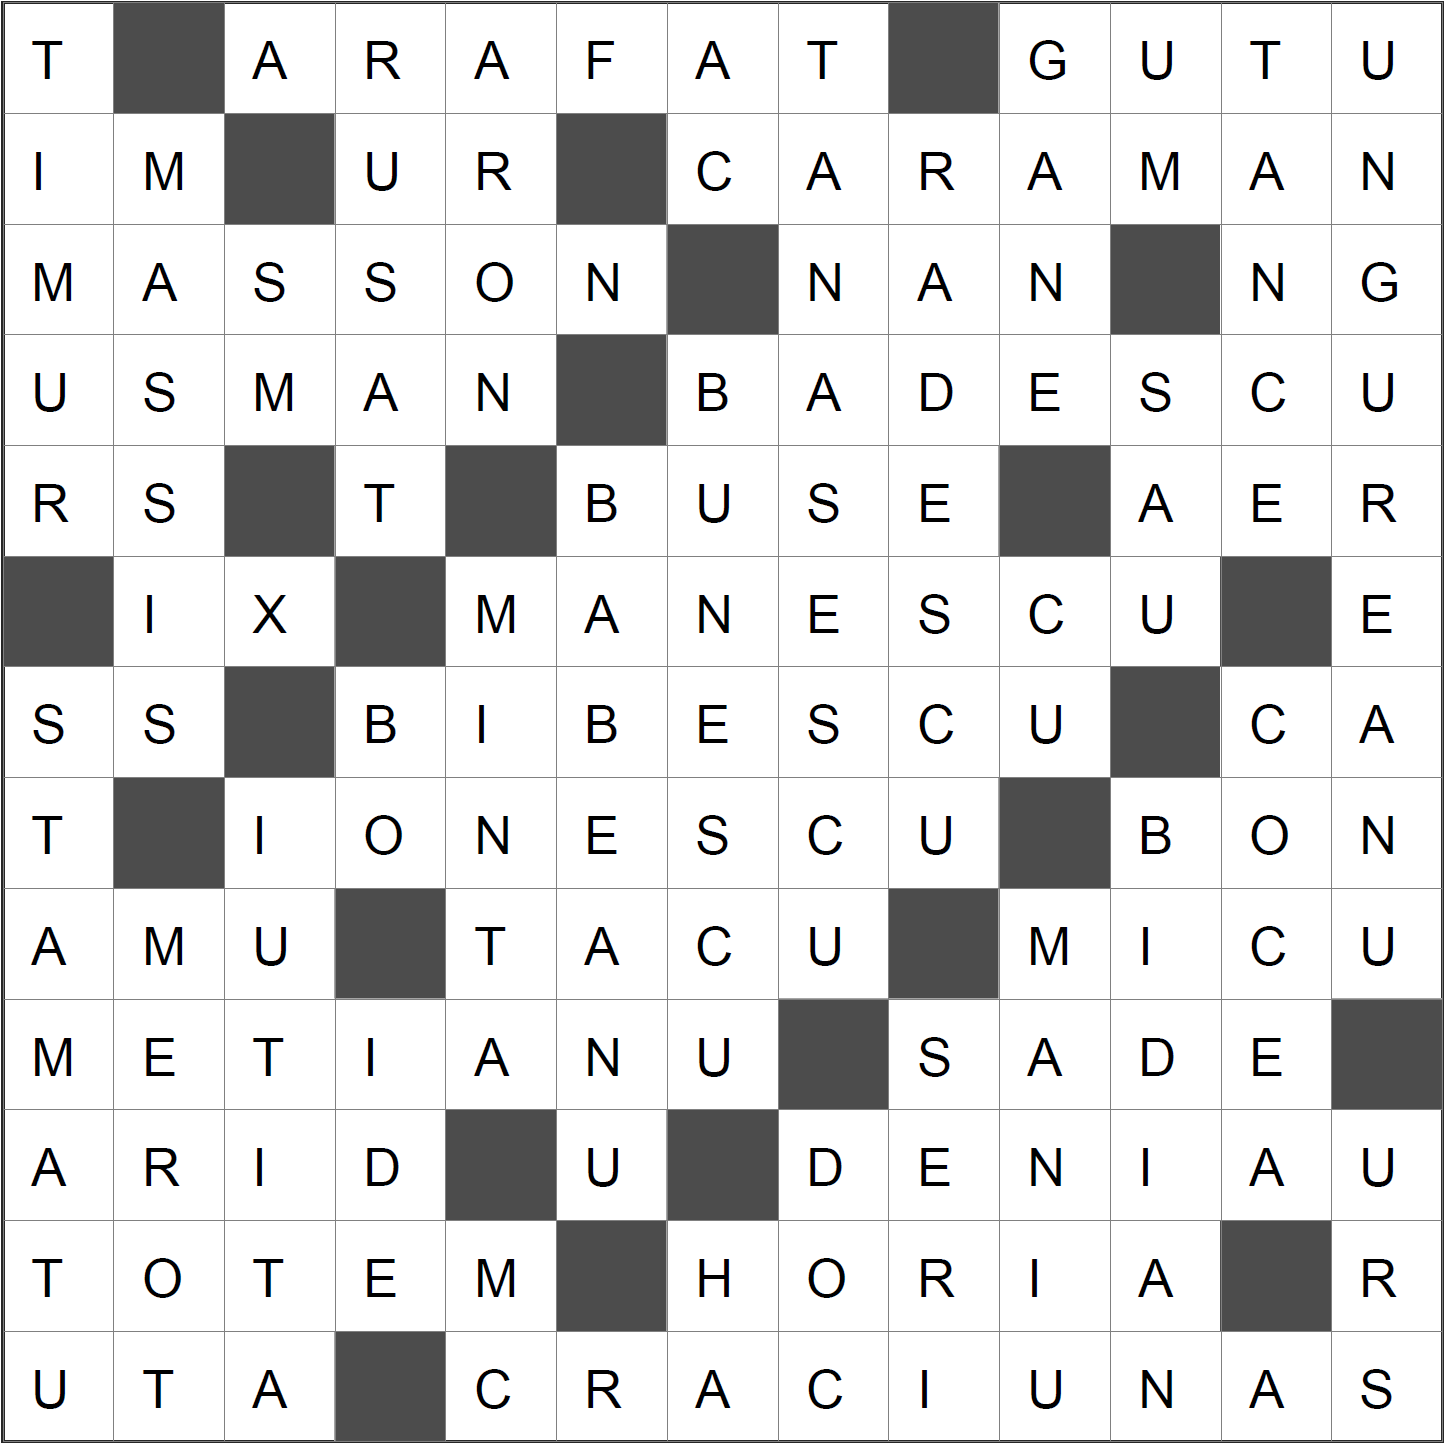
\includegraphics[height=3.1cm]{figs/2021b.png}
%
\hspace{1cm}
%
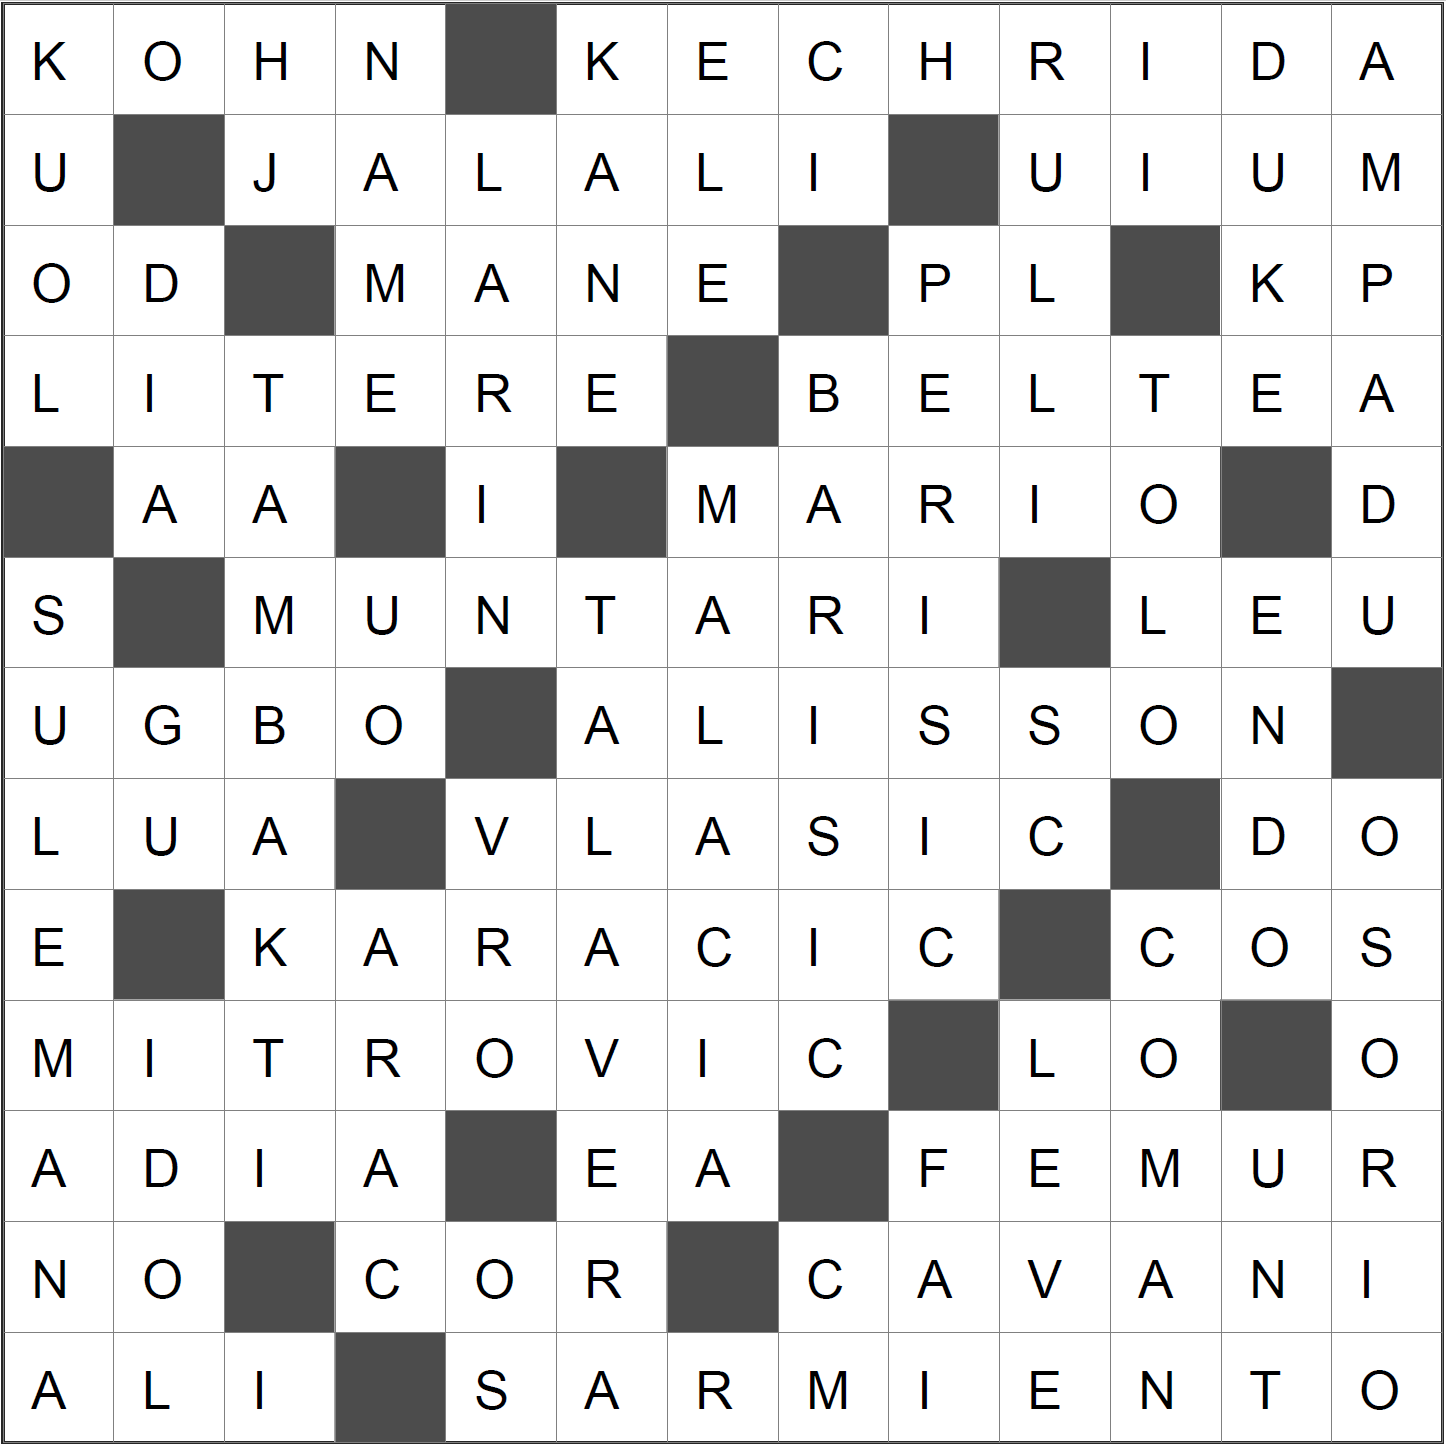
\includegraphics[height=3.1cm]{figs/2023b.png}

\caption{Our top results for years 2013 (left column), 2021 (middle column) and 2023 (right column). Top: seeds after placing additional black cells. Bottom: {\sc Wombat} solutions.}
\end{figure}

\end{frame}

%%%%%%%%%%%%%%%%%%%%%%%%%%%%%%%%%%%%%%%%%%%%%%%%%%%%%%%%%%%%%%%%%%%%%%%%%%%%%%%%

\begin{frame}{Scores}

\begin{table}[htbp]
\centering
\begin{tabular}{c|r|r|r}
\toprule
{\bf year} & {\bf human top-12 min} & {\bf human top-12 max} & {\bf our AI score} \\
\midrule
2013 & $175$ & $184$ & \tcg{$182$} \\ 
2021 & $187$ & $195$ & \tcg{$190$} \\ 
2023 & $183$ & $193$ & \tcg{$186$} \\ 
\bottomrule
\end{tabular}
\end{table}


\end{frame}



%%%%%%%%%%%%%%%%%%%%%%%%%%%%%%%%%%%%%%%%%%%%%%%%%%%%%%%%%%%%%%%%%%%%%%%%%%%%%%%%

\begin{frame}{Future Work}

\bei

\ie \tcm{Adi: please fill in a few bullets}

\bigskip

\ie \tcm{Adi: should we hit the conference attendees with our COG (6 out of 11 years) and post-COG (super-human performance) results here?}

\bigskip

\eei


\end{frame}


%%%%%%%%%%%%%%%%%%%%%%%%%%%%%%%%%%%%%%%%%%%%%%%%%%%%%%%%%%%%%%%%%%%%%%%%%%%%%%%%

\begin{frame}{Conclusions}

\bei

\ie {\sc Roco} is a difficult constraint optimization problem
\bei
\ie humans have been competing nationally from 1965
\ie AI was lagging behind
\eei

\medskip

\ie first human-competition-level AI performance in {\sc Roco}
\bei
\ie since then: super-human performance
\eei

\medskip

\ie our approach
\bei
\ie incrementally build and solve a constraint optimization problem
\ie start with a dense point-bearing cluster, build it up to a full solution
\ie pattern $\rightarrow$ core $\rightarrow$ expanded core $\rightarrow$ seed
\ie seed $\to$ solution
\bei
\ie one-shot completion for seed pre-selection
\ie incremental completion via stochastic search with explicit diversity 
\eei
\eei

\medskip
\medskip


\ie \tcb{acknowledgments: NSERC, CC, SoCS reviewers and J. Schaeffer}

\eei


\end{frame}

%%%%%%%%%%%%%%%%%%%%%%%%%%%%%%%%%%%%%%%%%%%%%%%%%%%%%%%%%%%%%%%%%%%%%%%%%%%%%%%%

\begin{frame}[allowframebreaks]{Bibliography}
\renewcommand*{\bibfont}{\footnotesize}
\printbibliography
\end{frame}

%%%%%%%%%%%%%%%%%%%%%%%%%%%%%%%%%%%%%%%%%%%%%%%%%%%%%%%%%%%%%%%%%%%%%%%%%%%%%%%%

\end{document}



